\chapter{Complejos Simpliciales}
En este capítulo introduciremos la noción de complejo simplicial y complejo simplicial abstracto, así como la relación entre ellos.
\section{Complejos Simpliciales en $\mathbb{R}^N$}
\subsection{Simplejos}  
El primer paso para definir un complejo simplicial, es estudiar las estructuras geométricas que lo conforman, es por ello que la primera parte de esta sección está dedicada a analizar los simplejos en $\mathbb{R}^N$.           
\begin{Defi}[Independencia Geométrica]
Dado un conjunto finito $\{a_0,..,a_n\}$ de puntos en $\mathbb{R}^{N}$, el conjunto es geométricamente independiente si la única solución al sistema 
\begin{equation}\label{s1}
    \begin{split}
     &\sum_{i=0}^{n}t_{i} = 0 \\
     &\sum_{i=0}^{n}t_{i}a_{i} = 0   
    \end{split}
\end{equation}

es $t_i = 0$ para toda $i$.
\end{Defi}

\begin{Teo}
\hspace{1cm}
\begin{enumerate}[(a)]
    \item El conjunto $\{a_0,...,a_n\}$ es geométricamente independiente si y sólo si $\{a_1-a_0,..,a_n-a_0\}$ es linealmente independiente.
    \item Si $\{a_0,...,a_n\}$ es geométricamente independiente entonces para todo subconjunto no vacío $A$ de $\{a_0,..,a_n\}$, $A$ es geométricamente independiente.
\end{enumerate}
\end{Teo}

\begin{Dem}
\begin{enumerate}[(a)]
\item Supongamos $\{a_0,...,a_n\}$ geométricamente independiente, si existe una combinación lineal de $\{a_1-a_0,...,a_n-a_0\}$ tal que $\sum_{i=1}^{n}t_i(a_i-a_0)=0$, reagrupando términos tenemos que $\sum_{i=1}^{n}t_ia_i + (-\sum_{i=1}^{n}t_i)a_0=0$, haciendo $t_0 = -\sum_{i=1}^{n}t_i$, se cumple \ref{s1}, al ser $\{a_0,...,a_n\}$ geométricamente independientes se tiene que $t_i=0$ para toda $i$.

Ahora supongamos que el conjunto $\{a_1-a_0,...,a_n-a_0\}$ es linealmente independiente, si $t_0,...,t_n$ son solución del sistema en \ref{s1}, entonces 
\begin{align*}
 0&=\sum_{i=0}^{n}t_ia_i\\
 &=\sum_{i=0}^{n}t_ia_i + -(\sum_{i=0}^{n}t_i)a_0\\
 &=\sum_{i=0}^{n}t_i(a_i-a_0)\\ 
 &= t_0(a_0-a_0) + \sum_{i=1}^{n}t_i(a_i-a_0)\\
 &=\sum_{i=1}^{n}t_i(a_i-a_0)
\end{align*}
Por lo tanto $t_i=0$ para toda $i$.
\item Basta demostrar que al quitarle un elemento al conjunto $\{a_0,...,a_n\}$
el conjunto resultante es geométricamente independiente, sin pérdida
de generalidad consideremos $\{a_0,...,a_n\}\backslash\{a_n\}$, por (a) tenemos que el
conjunto $\{a_1-a_0,...,a_n-a_0\}$ es linealmente independiente, y al quitarle
$a_n-a_0$ sigue siendo linealmente independiente y nuevamente por (a) 
tenemos que $\{a_0,...,a_n\}\backslash\{a_n\}$ es geométricamente independiente.
\end{enumerate}
\end{Dem}
Ejemplos:
\begin{enumerate}
\item Conjuntos de un solo punto
\item Tres puntos no colineales, cuatro puntos no coplanares y así sucesivamente.  
\item Todo conjunto linealmente independiente
\item Todo conjunto linealmente independiente unión con el vector cero. 
\end{enumerate}

\begin{Defi}[simplejo]
Sea $\{a_0,..,a_n\}$ un conjunto geométricamente independiente en  $\mathbb{R}^{N}$. Definimos el simplejo  $\sigma$ generado por $a_0,...,a_n$ como el conjunto de todos los puntos $x$ en $\mathbb{R}^{N}$ tales que 
\begin{equation}\label{s2}
\begin{split}
x = \sum_{i=0}^{n}t_ia_i,\\
\sum_{i=0}^{n}t_i=1
\end{split}
\end{equation}
con $t_i\geqslant 0$ para toda i.

Los puntos $a_0,...,a_n$ que generan a $\sigma$ son llamados los vértices de $\sigma$; y el número n la dimensión de $\sigma$.
\end{Defi}

\begin{figure}[h]
\centering
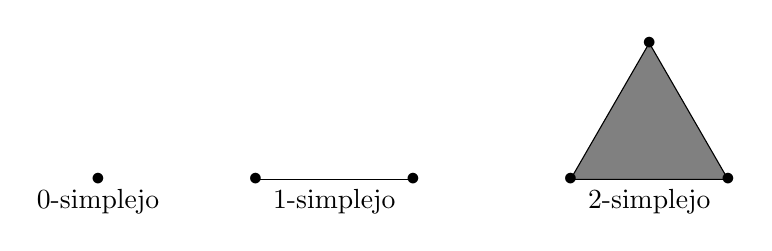
\begin{tikzpicture}
%\draw (-5,-5) grid (5,5);
\draw (-3,0) node {$\bullet$};
\draw (-3,0) node[below] {0-simplejo};

\draw (-1,0)--(1,0);
\draw (0,0) node[below] {1-simplejo};
\draw (-1,0) node {$\bullet$};
\draw (1,0) node {$\bullet$};

\draw [fill = gray] (3,0) -- (5,0) -- (4,1.73205) -- cycle;
\draw (3,0) node {$\bullet$};
\draw (5,0) node {$\bullet$};
\draw (4,1.73205) node {$\bullet$};
\draw (4,0) node[below] {2-simplejo};
\end{tikzpicture}
\caption{Ejemplos de simplejos}
\end{figure}

Notemos que para $x$ en $\sigma$ los coeficientes $t_i$ están determinados de manera única, ya que si $x = \sum_{i=0}^{n}t_ia_i$ y $x = \sum_{i=0}^{n}s_ia_i$ entonces los $t_i-s_i$ son solución del sistema \ref{s2} por lo que $t_i=s_i$ para toda $i$, lo que nos permite hacer la 
siguiente definición.
\begin{Defi}[Coordenadas baricéntricas]
Sea $\sigma$ un simplejo generado por $a_0,...,a_n$, si $x$ es un punto en $\sigma$, $x$ es de la forma $x = \sum_{i=0}^{n}t_ia_i$ con $t_i\geqslant 0$, las coordenadas baricéntricas $\{t_i(x):i = 0,..n\}$ del punto $x$ en $\sigma$ con respecto a $a_0,...,a_n$ se definen como funciones de $\sigma$ en $\mathbb{R}^{N}$ tales que $t_i(x) = t_i$
\end{Defi}

Veamos que las coordenadas baricéntricas $t_i(x)$ son continuas, para ello definamos la función $T$ de $\sigma$ en $\mathbb{R}^{N}$ como $T(x) = (t_0(x),...,t_n(x),0,...,0)$.
\begin{Prop}
T es continua.
\end{Prop}
\begin{Dem}

Sea $x$ un punto en $\sigma$, entonces $x=\sum_{i=0}^{n}t_i(x)a_i$ con $\sum_{i=0}^{n}t_i(x)=1$ y 
$t_i(x)\geq 0$, notemos que $t_0(x) = 1-\sum_{i=1}^{n}t_i(x)$ de donde se sigue que 
\begin{equation}
x = a_0 + \sum_{i=1}^{n}t_i(x)(a_i-a_0)
\end{equation}
El punto $x-a_0$ pertenece al espacio generado por $\{a_1-a_0,...,a_n-a_0\}$, los cuales son linealmente independientes y para $i>0$ las $t_i(x)$  son las coordendas de $x-a_0$ en la base $a_1-a_0,...,a_n-a_0$ por lo tanto son continuas y  como $t_0(x) = 1-\sum_{i=1}^{n}t_i(x)$ también es continua de donde se sigue la continuidad de T. 
\end{Dem}
Otras definiciones importantes sobre simplejos se enuncian a continuacion:
\begin{Defi}[Caras de un simplejo]
Sea $\sigma$ el simplejo generado por $a_0,a_1,...,a_n$ y $\tau$ un simplejo generado por algún subconjunto no vacío de $a_0,a_1,...,a_n$, decimos de $\tau$ es una cara de $\sigma$. Si $\tau$ está contenido estrictamente en $\sigma$ decimos que es una cara propia. 
\end{Defi}
\begin{Defi}[frontera e interior de un simplejo]
Sea $\sigma$ un simplejo, la frontera de $\sigma$ se define como la unión de todas sus caras propias y se denota por $Bd\sigma$. El interior de $\sigma$ se define como int $\sigma = \sigma-Bd\sigma$. 
\end{Defi}
\begin{Prop}
Para un simplex $\sigma$ generado por $a_0,...,a_n$ puntos en $\mathbf{R}^{N}$ se cumplen las siguientes propiedades:
\begin{enumerate}[(a)]
\item $\sigma$ es igual a la unión de todos los segmentos que unen a $a_0$ con los puntos del simplex $S$ generado por $a_1,...,a_n$.
\item $\sigma$ es un conjunto convexo y compacto en $\mathbf{R^{N}}$, el cual es igual a la intersección de todos los conjuntos convexos en $\mathbf{R^{N}}$ que contienen a $a_0,...,a_n$.
\item Dado un simplex $\sigma$ existe un único conjunto geométricamente independiente que lo genera.
\item Existe un homeomorfismo f de $\sigma$ en la bola unitaria $B^n$, tal que $Bd\sigma$ es mapeada a $B^n$, es decir $f(Bd\sigma) = S^{n-1}$.
\end{enumerate}
\end{Prop}

\section{Complejos en $\mathbb{R}^N$}
\begin{Defi}[Complejo Simplicial]
Un complejo simplicial $K$ en $\mathbb{R}^N$  es una colección de simplejos en $\mathbb{R}^N$ tal que:
\begin{enumerate}
\item Toda cara de un simplejo de K está en K.
\item La intersección de cualesquiera dos simplejos en K es una cara de cada una de ellas.
\end{enumerate}
\end{Defi}
\section{Complejos Simpliciales Abstractos}
A continuación introduciremos la noción de complejo simplicial abstracto y su relación con un complejo simplicial.
\begin{Defi}[Complejo simplicial abstracto]
Un complejo simplicial abstracto es una colección $\mathcal{S}$ de conjuntos no vacíos tales que si $A$ está en $\mathcal{S}$, todo subconjunto no vacío de $A$ también lo está.   
\end{Defi}
